\section{X-ray Summary}

X-rays are generated from the conversion of kinetic energy of electrons into electromagnetic radiation. To create the kinetic energy of the electrons, a element (tungsten cathode) is heated to release electrons into an electric potential field where a potential difference accelerates the electron toward the target anode and collides with the target material (tungsten).

When the electron hits that material and interacts with its nucleus, X-rays are formed. If the electron hits the nucleus, the x-ray that is produced has maximal energy. If the electron passes within close proximity to a nucleus, an x-ray is still generated but the energy is lower.  The farther the electron is from a nucleus, the lower the energy.  The spectrum of the energy distribution is called the bremsstrahalung spectrum, seen in figure \ref{fig:brem}.  The spikes in this figure labeled characteristic radiation come from when an incident electron has enough energy to remove an electron from a target material atom, the creating an empty electron spot.  Another electron then moves into this empty location from an outer shell, which releases characteristic radiation which is specific to the location of the electron that was removed. 

\begin{figure}[h]
	\centering
	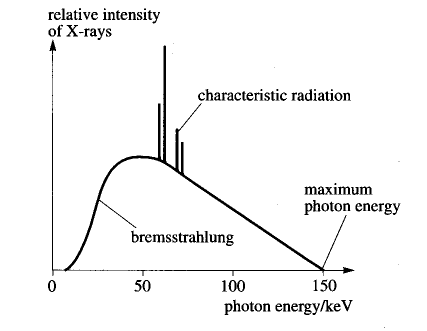
\includegraphics[width=0.7\linewidth]{bramSpec}
	\caption{Bremsstrahalung Spectrum}
	\label{fig:brem}
\end{figure}

\section{Projections and Reconstructions}

The basic equation for taking a projection of an object at a given angle is the following:

\begin{equation}
g(\rho_i,\theta_k) = \int_{-\infty}^{\infty} \int_{-\infty}^{\infty} I(x,y) \; \delta \big(xcos(\theta) + ysin(\theta) - \rho \big) \; dx \; dy
\label{eq:Radon}
\end{equation}

\noindent
where $g(\rho_i,\theta_k)$ is the radon transform for given sets $\{\rho_i\}$ and $\{\theta_k\}$, $I(x,y)$ is the image that is desired image, or the object, and $\delta$ is the dirac delta function. Back projection then uses these individual projections to create a final image.  For a given $\theta$ the back-projected image is the following:

\begin{equation}
f_{\theta}(x,y) = g(xcos(\theta) + ysin(\theta), \theta)
\end{equation}

\noindent
Summation of these individual back-projected images generates a final image of the original object:

\begin{equation}
I(x,y) = \sum_{\theta=0}^{\pi} \: f_{\theta}(x,y) = \sum_{\theta=0}^{\pi} \: g(xcos(\theta) + ysin(\theta), \theta)
\end{equation}

However this causes blurring due to multiple projections adding up in the middle (over-sampling), which means that the image obtained is not correct. What is needed is filtered back projection.  A key theorem for this is the central slice theorem which states that the 1-D Fourier transform of a radon transform is a single slice of the 2-D Fourier transform of the image that passes through the origin at angle $\theta$. To prove this, let us consider a single radon transform at angle $\theta$ and take the 1-D Fourier transform of it:

\begin{equation}
G(w,\theta) = \int_{-\infty}^{\infty} g(\rho,\theta) \: e^{i2\pi  w \rho} \: d\rho
\label{eq:1Dft}
\end{equation}

\noindent
substituting \ref{eq:Radon} into \ref{eq:1Dft} yeilds the following:

\begin{equation}
G(w,\theta) = \int_{-\infty}^{\infty} \: \biggl[  \int_{-\infty}^{\infty} \int_{-\infty}^{\infty} I(x,y) \; \delta \big(xcos(\theta) + ysin(\theta) - \rho \big) \; dx \; dy  \biggr] \: e^{i2\pi  w \rho} \: d\rho
\end{equation}

\noindent
rearranging this gives:

\begin{equation}
G(w,\theta) = \int_{-\infty}^{\infty} \int_{-\infty}^{\infty} I(x,y) \: \biggl[ \underbrace{ \int_{-\infty}^{\infty} \delta \big(xcos(\theta) + ysin(\theta) - \rho \big) e^{i2\pi w \rho} \: d\rho} \biggr] \: dx \: dy
\end{equation}

\noindent
using the properties of the dirac delta, the equation can be simplified:

\begin{equation}
G(w,\theta) = \int_{-\infty}^{\infty} \int_{-\infty}^{\infty} I(x,y)   e^{i2\pi w \big(xcos(\theta) + ysin(\theta) \big)} \: dx \: dy \: = \: F(wcos(\theta),wsin(\theta))
\label{eq:sliceThrm}
\end{equation}

\noindent
 Note that this is the a slice of the 2-D Fourier transform along a line $w$ at angle $\theta$. Let us now look at reconstructing the desired image from the Fourier space:

\begin{equation}
I(x,y) = \int_{-\infty}^{\infty} \int_{-\infty}^{\infty} F(u,v)   e^{i2\pi \big(ux + vy \big)} \: du \: dv 
\end{equation}

\noindent 
Now we can convert this to polar coordinates:

\begin{equation}
I(x,y) = \int_{0}^{2\pi} \int_{-\infty}^{\infty} w \: F(wcos(\theta),wsin(\theta))   e^{i2\pi w\big(xcos(\theta) + ysin(\theta) \big)} \:  dw \: d\theta
\end{equation}

\noindent
Using the Fourier slice theorm from \ref{eq:sliceThrm} we can write the following:

\begin{equation}
I(x,y) = \int_{0}^{2\pi} \int_{-\infty}^{\infty} w\:  G(w,\theta)  e^{i2\pi w\big(xcos(\theta) + ysin(\theta) \big)} \:  dw \: d\theta
\end{equation}

\noindent
Here we can note that $G(w,\theta + \pi) = G(-w,\theta)$ so we can write the following:

\begin{equation}
I(x,y) = \int_{0}^{\pi} \int_{-\infty}^{\infty} |w|\: G(w,\theta)  e^{i2\pi w\big(xcos(\theta) + ysin(\theta) \big)} \:  dw \: d\theta
\end{equation}

What this shows is that the desired image needs to have the 1-D Fourier transforms of the projections each filtered by $|w|$ in order properly reconstruct the image. This is called filtered back projection and now that the individual projections have been scaled, the reconstructed image is now correct. 

\section{Sampling Criteria}